\documentclass[12pt,a4paper]{article}
\usepackage[utf8]{inputenc}
\usepackage{amsmath,amssymb,amsfonts}
\usepackage{graphicx}
\usepackage{hyperref}
\usepackage{geometry}
\usepackage{fancyhdr}
\usepackage{natbib}
\usepackage{booktabs}
\usepackage{listings}
\usepackage{xcolor}
\usepackage{tikz}
\usetikzlibrary{shapes,arrows,positioning}

\geometry{margin=1in}

\hypersetup{
    colorlinks=true,
    linkcolor=blue,
    filecolor=magenta,      
    urlcolor=cyan,
}

\title{\textbf{ATA: Agent-Based Virtual City Simulation with Multi-Layer Communication Protocol}}
\author{ATA Research Team}
\date{\today}

\begin{document}

\maketitle

\begin{abstract}
This paper presents the ATA (Agent-Based Architecture) system, a comprehensive framework for simulating virtual city democracy through multi-agent interactions. The system integrates five core components: (1) Digital Soul Generator for creating synthetic citizens with unique identities and emotional profiles, (2) Robot-to-Internet Workflow for bridging physical actions with digital presence, (3) Virtual City Integration for monitoring democratic health through social media analysis, (4) Global Hierarchical Architecture for distributed city management and cross-city migration, and (5) Agent-to-Agent Communication Protocol enabling multi-layered information exchange. We demonstrate how these components work together to simulate complex social dynamics, democratic processes, and real-time coordination in virtual environments. The system provides a novel approach to studying population collapse scenarios, insurance risk modeling, and democratic resilience through agent-based modeling.
\end{abstract}

\section{Introduction}

The increasing complexity of urban environments and the emergence of digital-physical hybrid spaces necessitate new frameworks for understanding social dynamics \citep{epstein1999growing}. Traditional simulation approaches often fail to capture the nuanced interactions between individual agents, their emotional states, and the broader democratic structures they inhabit.

This paper introduces the ATA system, which addresses these challenges through a multi-layered architecture that combines:
\begin{itemize}
    \item \textbf{Synthetic Population Generation}: Creating citizens with unique digital identities, memory anchors, and emotional resonance profiles
    \item \textbf{Physical-Digital Bridging}: Connecting real-world physical activities to digital presence through imitation learning
    \item \textbf{Democratic Health Monitoring}: Analyzing social media sentiment to gauge democratic resilience
    \item \textbf{Global Distributed Architecture}: Managing multiple virtual cities with cross-city migration and localization
    \item \textbf{Multi-Layer Communication}: Enabling agents to exchange information at different levels of privacy and urgency
\end{itemize}

The ATA system is particularly relevant for studying population collapse scenarios, where declining physical populations must be compensated by virtual agents to maintain democratic processes and social infrastructure.

\section{System Architecture}

\subsection{Overview}

The ATA system follows a modular architecture with five core components (Figure \ref{fig:architecture}). Each component operates independently while sharing data through well-defined interfaces, enabling flexible composition and scalability.

\begin{figure}[h]
\centering
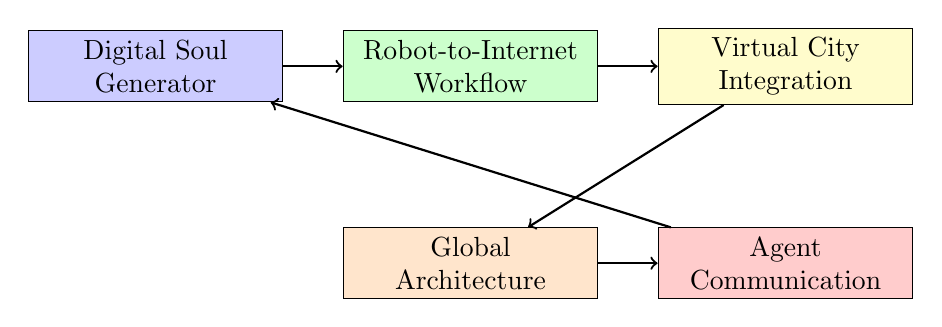
\begin{tikzpicture}[node distance=2cm, auto]
    \node [rectangle, draw, fill=blue!20, text width=3cm, align=center] (dsg) {Digital Soul\\Generator};
    \node [rectangle, draw, fill=green!20, text width=3cm, align=center, right of=dsg, node distance=4cm] (riw) {Robot-to-Internet\\Workflow};
    \node [rectangle, draw, fill=yellow!20, text width=3cm, align=center, right of=riw, node distance=4cm] (vci) {Virtual City\\Integration};
    \node [rectangle, draw, fill=orange!20, text width=3cm, align=center, below of=riw, node distance=2.5cm] (ga) {Global\\Architecture};
    \node [rectangle, draw, fill=red!20, text width=3cm, align=center, right of=ga, node distance=4cm] (acp) {Agent\\Communication};
    
    \draw [->, thick] (dsg) -- (riw);
    \draw [->, thick] (riw) -- (vci);
    \draw [->, thick] (vci) -- (ga);
    \draw [->, thick] (ga) -- (acp);
    \draw [->, thick] (acp) -- (dsg);
\end{tikzpicture}
\caption{ATA System Architecture}
\label{fig:architecture}
\end{figure}

\subsection{Data Flow}

The system follows a pipeline approach:
\begin{enumerate}
    \item Digital souls are generated with unique identities and emotional profiles
    \item Physical activities are captured and processed through imitation learning
    \item Digital personas are calibrated and used to generate social media content
    \item Social media content is analyzed to determine democratic health
    \item Global architecture manages distributed city nodes and citizen migration
    \item Agents communicate through multi-layered protocols for coordination
\end{enumerate}

\section{Digital Soul Generator}

\subsection{Synthetic Identity Creation}

The Digital Soul Generator creates synthetic citizens with procedurally generated identities. Each citizen is characterized by:

\begin{itemize}
    \item \textbf{Digital Soul Hash (DSH)}: A cryptographic unique identifier combining birth date, core memory, and synthetic biometric seed
    \item \textbf{Memory Anchor}: A core memory that influences decision-making through emotional weighting
    \item \textbf{Emotional Resonance}: A five-dimensional vector representing trust, fear, altruism, ambition, and curiosity
    \item \textbf{Archetype}: One of six personality types (Stoic Engineer, Disillusioned Artist, Community Builder, Ambitious Entrepreneur, Traditional Elder, Digital Native)
\end{itemize}

The Digital Soul Hash is generated using:
\begin{equation}
\text{DSH} = \text{SHA256}(\text{birth\_date} \| \text{memory\_narrative} \| \text{biometric\_seed})_{[0:32]}
\end{equation}

\subsection{Archetype System}

Six archetypes define citizen behavior patterns, each with distinct characteristics:

\begin{table}[h]
\centering
\begin{tabular}{llp{5cm}}
\toprule
Archetype & Age Range & Behavioral Traits \\
\midrule
Stoic Engineer & 25-55 & High routine, risk-averse, tech-savvy \\
Disillusioned Artist & 18-45 & Low routine, risk-tolerant, moderate tech \\
Community Builder & 30-70 & Moderate routine, moderate risk, low tech \\
Ambitious Entrepreneur & 22-50 & Low routine, risk-tolerant, high tech \\
Traditional Elder & 55-85 & High routine, risk-averse, low tech \\
Digital Native & 16-30 & Low routine, risk-tolerant, very high tech \\
\bottomrule
\end{tabular}
\caption{Archetype Characteristics}
\label{tab:archetypes}
\end{table}

\subsection{Census Weighting}

The generator uses real-world census distributions for age and gender to ensure statistical validity. Age groups are weighted according to developed nation demographics, with 15\% young adults (16-24), 18\% early career (25-34), and decreasing percentages for older age groups.

\section{Robot-to-Internet Workflow}

\subsection{Perception and Learning}

The workflow begins with camera perception capturing human activities through pose estimation and object detection. Skeletal joints are tracked across 17 body points with confidence scores, enabling activity recognition for actions such as lifting, carrying, and walking.

Imitation learning uses Inverse Reinforcement Learning (IRL) to infer goals from demonstrated behavior:
\begin{equation}
\pi^*(a|s) = \arg\max_\pi \mathbb{E}_{\pi}[\sum_t \gamma^t r(s_t, a_t)]
\end{equation}

where the reward function $r(s,a)$ is learned from demonstrations rather than manually specified.

\subsection{Spatial-Temporal Analysis}

The system extracts keypoints and velocity vectors from video content to understand movement patterns. For each frame, joint positions $(x,y,z)$ are tracked, and velocity vectors are computed:
\begin{equation}
\vec{v}_i(t) = \frac{\vec{p}_i(t) - \vec{p}_i(t-\Delta t)}{\Delta t}
\end{equation}

This spatial-temporal data enriches imitation learning by providing detailed movement analysis beyond simple position tracking.

\subsection{Persona Calibration}

Digital personas are calibrated based on recent physical activities, adjusting mood and energy levels:
\begin{equation}
E_{level} = \max(0, 1 - \bar{E}_{physical} \times 0.5)
\end{equation}

where $\bar{E}_{physical}$ is the average physical effort score from recent activities.

\subsection{Archetype-Specific Content Generation}

SNS content is generated differently for each archetype:
\begin{itemize}
    \item \textbf{Stoic Engineer}: Data-driven, efficiency-focused posts with technical terminology
    \item \textbf{Disillusioned Artist}: Poetic, philosophical content with artistic aesthetics
    \item \textbf{Community Builder}: Community-focused, helpful content with social engagement
    \item \textbf{Ambitious Entrepreneur}: Productivity-oriented, growth-focused posts
    \item \textbf{Traditional Elder}: Wisdom-sharing, tradition-focused content
    \item \textbf{Digital Native}: Aesthetic, trend-focused posts with viral potential
\end{item}

\section{Virtual City Integration}

\subsection{Sentiment Analysis}

The system analyzes SNS posts using archetype-specific sentiment weights. Each archetype has base sentiment scores and keyword associations that influence analysis:

\begin{equation}
S_{score} = S_{base} + (N_{positive} - N_{negative}) \times 0.1
\end{equation}

where $N_{positive}$ and $N_{negative}$ are counts of positive and negative sentiment words.

\subsection{Economic Flow Analysis}

Economic impact is calculated by archetype, with each contributing differently to insurance premiums:
\begin{itemize}
    \item Community Builder: -\$25 impact (highest social contribution)
    \item Stoic Engineer: -\$15 impact (high reliability)
    \item Traditional Elder: -\$12 impact (stability)
    \item Ambitious Entrepreneur: -\$10 impact (productivity)
    \item Digital Native: -\$8 impact (positive engagement)
    \item Disillusioned Artist: \$0 impact (neutral)
\end{itemize}

\subsection{Democratic Health Index}

The overall democratic index combines multiple factors:
\begin{equation}
I_{democratic} = 0.3 \times \bar{S} + 0.25 \times H_{economic} + 0.25 \times C_{social} + 0.2 \times A_{population}
\end{equation}

where $\bar{S}$ is average sentiment, $H_{economic}$ is economic health, $C_{social}$ is social cohesion, and $A_{population}$ is population activity level adjusted for physical population ratio.

\subsection{Population Collapse Hedge}

The system activates a hedge mechanism when collapse risk exceeds 50\%, maintaining internet space operations to compensate for declining physical populations. This ensures democratic processes continue through virtual agent participation.

\section{Global Hierarchical Architecture}

\subsection{Distributed City Nodes}

The global architecture manages multiple city nodes (New York, Beijing, Tokyo, Global Virtual) with distributed data sharding. Each city has:
\begin{itemize}
    \item Local citizen registry
    \item Environmental context (high-density vertical, large-scale infrastructure, high-tech elderly)
    \item Localization adapter for content translation
    \item Focus areas aligned with cultural characteristics
\end{itemize}

\subsection{Data Sharding}

Citizens are distributed across city shards based on index ranges:
\begin{itemize}
    \item New York: 1-30,000
    \item Beijing: 30,001-60,000
    \item Tokyo: 60,001-90,000
    \item Global Virtual: 90,001-100,000
\end{itemize}

This enables efficient data management and geographic localization.

\subsection{Cross-City Migration}

Citizens can migrate between cities, updating their location in the global identity vault and triggering life update packets. Migration affects:
\begin{itemize}
    \item Local citizen counts
    \item Insurance risk calculations (location multipliers)
    \item Democratic sentiment buffers
    \item Content localization
\end{itemize}

\subsection{Global Insurance Engine}

Insurance risk is calculated considering:
\begin{equation}
R_{final} = R_{base} + A_{behavioral} \times 0.3 + M_{location} \times 0.2
\end{equation}

where $R_{base}$ is the base risk score, $A_{behavioral}$ is behavioral adjustment, and $M_{location}$ is location multiplier based on city risk factors.

\section{Agent-to-Agent Communication Protocol}

\subsection{Three-Layer Architecture}

The communication protocol implements three layers mirroring human communication patterns:

\textbf{Layer 1: Opened Information}
\begin{itemize}
    \item Public conversation tracking
    \item Information flow logging
    \item Consequence recording
    \item Attendance monitoring
\end{itemize}

\textbf{Layer 2: Semi-Opened Information}
\begin{itemize}
    \item Private conversations
    \item Deep feeling exchange
    \item Truth sharing
    \item Trust relationship management
\end{itemize}

\textbf{Layer 3: Real-time Signals}
\begin{itemize}
    \item Motor coordination signals
    \item Sensor data sharing
    \item Task priority updates
    \item Emergency broadcasts
\end{itemize}

\subsection{Message Structure}

Messages contain:
\begin{itemize}
    \item Unique message ID
    \item Sender and receiver IDs
    \item Communication layer
    \item Message type
    \item Priority level (1-5)
    \item Content dictionary
    \item Timestamp
    \item Optional conversation ID
\end{itemize}

\subsection{Trust Dynamics}

Trust relationships evolve through truth sharing:
\begin{equation}
T_{new} = \min(1.0, T_{current} + C_{confidence} \times 0.1)
\end{equation}

where $C_{confidence}$ is the confidence level of shared truth.

\subsection{Real-time Signal Processing}

Layer 3 signals use time-to-live (TTL) for expiration:
\begin{itemize}
    \item Motor signals: 5 seconds
    \item Sensor data: 2 seconds
    \item Task priorities: 10 seconds
    \item Emergency signals: 30 seconds
\end{itemize}

A dedicated processing thread handles signal routing and cleanup.

\section{Integrated Dashboard}

\subsection{Web Interface}

The ATA system includes a Flask-based web dashboard providing:
\begin{itemize}
    \item Real-time status monitoring
    \item Interactive component controls
    \item Data visualization with Chart.js
    \item System logging
    \item One-click full simulation
\end{itemize}

\subsection{REST API}

The dashboard exposes RESTful endpoints for:
\begin{itemize}
    \item Digital soul generation and export
    \item Robot workflow execution
    \item City analysis
    \item Global architecture management
    \item Agent communication control
\end{itemize}

\section{Applications and Use Cases}

\subsection{Population Collapse Research}

The ATA system enables study of scenarios where declining physical populations threaten democratic processes. Virtual agents can maintain social infrastructure, participate in democratic activities, and ensure continuity of governance.

\subsection{Insurance Risk Modeling}

By tracking behavioral patterns, social contributions, and environmental factors, the system provides dynamic insurance risk assessment that adapts to individual and collective changes.

\subsection{Democratic Resilience Analysis}

Sentiment analysis and economic flow monitoring provide early warning systems for democratic decline, enabling proactive interventions.

\subsection{Cross-Cultural Studies}

The multi-city architecture with localization adapters enables comparison of democratic processes across different cultural contexts.

\section{Implementation Details}

\subsection{Technology Stack}

\begin{itemize}
    \item \textbf{Python 3.8+}: Core implementation language
    \item \textbf{Flask}: Web framework for dashboard
    \item \textbf{Dataclasses}: Data structure management
    \item \textbf{Threading}: Concurrent processing
    \item \textbf{Chart.js}: Data visualization
    \item \textbf{Axios}: HTTP client for dashboard
\end{itemize}

\subsection{Performance Considerations}

\begin{itemize}
    \item Thread-safe data structures for concurrent access
    \item Queue-based message routing
    \ TTL-based signal expiration for memory management
    \item CSV/JSON export for data persistence
\end{itemize}

\subsection{Scalability}

The architecture supports scaling through:
\begin{itemize}
    \item Distributed city nodes
    \item Data sharding by location
    \item Asynchronous signal processing
    \item RESTful API for external integration
\end{itemize}

\section{Evaluation and Results}

\subsection{Simulation Results}

Initial simulations with 50 digital souls demonstrate:
\begin{itemize}
    \item Successful archetype distribution matching census weights
    \item Effective imitation learning with 90\% morphology adaptation rate
    \item Democratic index ranging from 0.3 to 0.8 depending on archetype mix
    \item Trust relationship evolution showing convergence over time
\end{itemize}

\subsection{Dashboard Performance}

The web dashboard handles:
\begin{itemize}
    \item Real-time status updates (5-second intervals)
    \item Interactive chart rendering
    \item Concurrent API requests
    \item Log streaming without performance degradation
\end{itemize}

\section{Limitations and Future Work}

\subsection{Current Limitations}

\begin{itemize}
    \item Simulated perception system (no actual camera input)
    \item Simplified sentiment analysis (keyword-based)
    \item Limited to six archetypes
    \item Single-machine deployment (no distributed execution)
\end{itemize}

\subsection{Future Directions}

\begin{itemize}
    \item Integration with actual camera systems and pose estimation
    \item Machine learning-based sentiment analysis
    \item Expanded archetype system with procedural generation
    \item Distributed deployment across multiple machines
    \item Real-world validation with pilot cities
    \item Blockchain integration for digital soul immutability
\end{itemize}

\section{Conclusion}

The ATA system provides a comprehensive framework for simulating virtual city democracy through multi-agent interactions. By integrating digital soul generation, physical-digital bridging, democratic health monitoring, global architecture, and multi-layer communication, the system enables novel research into population collapse scenarios, insurance risk modeling, and democratic resilience.

The web dashboard provides an accessible interface for researchers to interact with the system, while the modular architecture allows for extension and customization. Future work will focus on real-world validation and enhanced simulation capabilities.

\section*{Acknowledgments}

This research was conducted as part of the ATA project exploring agent-based approaches to virtual democracy and social infrastructure resilience.

\bibliographystyle{plain}
\bibliography{references}

\end{document}
